\documentclass[a4paper,12pt]{report}
\usepackage[utf8]{vietnam}
\usepackage{amsmath}
\usepackage{amsmath}
\usepackage{amsfonts}
\usepackage{amssymb}
\usepackage{graphicx}
\usepackage{fancybox}
\usepackage{longtable}
\usepackage{listings}
\usepackage[left=3cm, right=2.00cm, top=2.00cm, bottom=2.00cm]{geometry}
\lstset{
   %keywords={break,case,catch,continue,else,elseif,end,for,function,
   %   global,if,otherwise,persistent,return,switch,try,while},
   basicstyle=\ttfamily \fontsize{12}{15}\selectfont,   
	% numbers=left,
   frame=lrtb,
tabsize=3
}
\PassOptionsToPackage{hyphens}{url}\usepackage{hyperref}  
\usepackage{float}
\hypersetup{
    colorlinks,
    citecolor=black,
    filecolor=black,
    linkcolor=black,
    urlcolor=black
}
\setlength{\parskip}{0.6em}
\usepackage[nottoc]{tocbibind}
\usepackage[english]{babel}
\addto\captionsenglish{%
 \renewcommand\chaptername{Phần}
 \renewcommand{\contentsname}{Mục lục} 
 \renewcommand{\listtablename}{Danh sách bảng}
 \renewcommand{\listfigurename}{Danh sách hình vẽ}
 \renewcommand{\tablename}{Bảng}
 \renewcommand{\figurename}{Hình}
 \renewcommand{\bibname}{Tài liệu tham khảo}
}

\begin{document}
\thispagestyle{empty}
\thisfancypage{
\setlength{\fboxrule}{1pt}
\doublebox}{}
\begin{center}
{\fontsize{16}{19}\fontfamily{cmr}\selectfont TRƯỜNG ĐẠI HỌC BÁCH KHOA HÀ NỘI\\
VIỆN CÔNG NGHỆ THÔNG TIN VÀ TRUYỀN THÔNG}\\
\textbf{------------*******---------------}\\[1cm]

\includegraphics[scale=0.13]{hust.jpg}\\[1.3cm]

{\fontsize{32}{43}\fontfamily{cmr}\selectfont BÁO CÁO}\\[0.1cm]
{\fontsize{38}{45}\fontfamily{cmr}\fontseries{b}\selectfont MÔN HỌC}\\[0.2cm]
{\fontsize{19}{20}\fontfamily{phv}\selectfont Xử lý ngôn ngữ tự nhiên}\\[0.2cm]
{\fontsize{13}{20}\fontfamily{cmr}\selectfont \emph{Đề tài: Phân tích quan điểm}}\\[2.5cm]
\end{center}
\hspace{1.5cm}\fontsize{14}{16}\fontfamily{cmr}\selectfont \textbf{Nhóm sinh viên thực hiện:}

\begin{longtable}{l c c}

Họ và tên & MSSV  & Lớp\\

Nguyễn Tuấn Đạt & 20130856 & CNTT2.02-K58 \\
Phan Anh Tú &   20134501 & CNTT2.01-K58\\

\end{longtable}

\hspace{1cm}\fontsize{14}{16}\fontfamily{cmr}\selectfont \textbf{Giáo viên hướng dẫn: }PGS.TS Lê Thanh Hương \\[2cm]
\begin{center}
\fontsize{16}{19}\fontfamily{cmr}\selectfont Hà Nội 12--2016

\end{center}
\newpage
\pdfbookmark{\contentsname}{toc}
\tableofcontents
%\listoftables
\listoffigures

\chapter*{Lời cảm ơn}
\phantomsection
\addcontentsline{toc}{chapter}{Lời cảm ơn}
Đề tài sẽ không thể hoàn thành nếu không nhờ có sự tận tình chỉ bảo và hướng dẫn của cô giáo PGS.TS Lê Thanh Hương. Mặc dù đã rất cố gắng để hoàn thành tốt nhưng trong quá trình làm việc, sai sót là điều không thể tránh khỏi. Nhóm chúng em mong nhận được nhận xét và phê bình của quý thầy cô để đề tài được hoàn thiện hơn đồng thời bổ sung những kiến thức còn thiếu sót cho chúng em.


Chúng em xin chân thành cảm ơn!

\chapter{Đặt vấn đề }
Cùng với sự phát triển mạnh mẽ của ngành công nghệ thông tin và truyền thông, trí tuệ nhân tạo đang ngày càng phát triển và có thể nói trong tương lai không xa máy tính sẽ trở nên thông minh chẳng kém gì con người. Trong trí tuệ nhân tạo thì hai mảng học máy và xử lý ngôn ngữ tự nhiên là hai mảng tiềm năng và phát triển cực mạnh, là hai trong số rất nhiều mảng của trí tuệ nhân tạo được tập trung nghiên cứu nhiều nhất hiện nay.


Là những sinh viên ngành công nghệ thông tin, là một kỹ sư công nghệ thông tin trong tương lai, chúng em nhận thấy cần phải trang bị cho mình những kiến thức nền tảng và những kinh nghiệm trong các bài toán thực tế về các mảng xử lý ngôn ngữ tự nhiên và học máy. Vì vậy, mục tiêu của bài tập lớn môn học này của chúng em là tìm hiểu lý thuyết và ứng dụng các kỹ thuật học máy cụ thể là hai phương pháp: \textbf{Support Vector Machine (SVM)} và \textbf{Long Short Term Memory (LSTM)} vào bài toán phân tích quan điểm của mảng xử lý ngôn ngữ tự nhiên.


Các nội dung triển khai trong đề tài này được thực hiện theo nhóm gồm hai sinh viên bao gồm: Nguyễn Tuấn Đạt và Phan Anh Tú. Trong đó dưới sự hướng dẫn của cô giáo PGS.TS Lê Thanh Hương, mỗi người phụ trách một số nội dung tách biệt nhau:
\begin{enumerate}
\item Nguyễn Tuấn Đạt
\begin{itemize}
\item Tìm hiểu và cài đặt SVM
\end{itemize}
\item Phan Anh Tú
\begin{itemize}
\item Tìm hiểu và cài đặt RNN,LSTM
\end{itemize}
\end{enumerate}
Phần tiếp theo của báo cáo bao gồm các phần sau:
\par Phần 2: Trình bày tóm lược về lý thuyết cách biểu diễn dữ liệu; các phương pháp học máy áp dụng: SVM, LSTM.
\par Phần 3: Giới thiệu bài toán thực tế áp dụng và kết quả thực nghiệm với các phương pháp học máy (SVM, LSTM).
\par Phần 4: Trình bày khó khăn gặp phải trong quá trình thực hiện đề tài và hướng phát triển trong tương lai.

\chapter{Cơ sở lý thuyết}
\section{Biểu diễn dữ liệu}
Trong khi máy tính chỉ làm việc (tính toán) với các con số, các vector. Làm thế nào để máy tính có thể hiểu được ngôn ngữ tự nhiên. Phần này chúng em sẽ đề cập đến một số mô hình biểu diễn dữ liệu từ dạng text sang vector số, cụ thể là biểu diễn các từ trong ngôn ngữ tự nhiên thành các vector số (word embedding).
 
\subsection{One-hot vector}
Mô hình này biểu diễn mỗi từ thành một vector có số chiều là độ dài của từ điển ($\mathbb{R}^{|V|\times 1}$ ($|V|$ là kích thước của từ điển)). Tất cả các phần tử của vector one-hot của một từ có giá trị bằng 0 ngoại trừ vị trí của từ đó trong từ điển trong vector có giá trị bằng 1. Ví dụ từ \emph{a} là từ đầu tiên trong từ điển thì vector biểu diễn từ \emph{a} có dạng $w^a = [1,0,0,...,0]$
\par Mô hình này sẽ biểu diễn các từ độc lập với nhau, 2 từ có có nghĩa tương tự nhau cũng bị xem như là khác nhau. Ví dụ độ tương đồng giữa 2 từ \emph{hotel} và \emph{motel} bằng với độ tương đồng giữa 2 từ \emph{hotel} và \emph{cat} (do $(w^{hotel})^Tw^{motel} = (w^{hotel})^Tw^{cat} = 0$)
\par Mặt khác nếu kích thước của từ điển lớn thì sẽ gây lãng phí bộ nhớ khi biểu diễn một từ là vector có số chiều là độ dài của từ điển.

\subsection{Mô hình dựa trên phương pháp lặp}
Các mô hình này cho phép dự đoán các từ dựa trên ngữ cảnh (context) của nó. Một context $C$ của một từ trong một câu là tập $C$ từ xung quanh nó. Ví dụ câu:\\
\centerline{\emph{"The cat jumped over puddle"}}\\[0.2cm]
C = 2 context của từ \emph{"jumped"} (center word) là tập \{ \emph{"the", "cat", "over", "puddle"} \}.

\subsubsection{Mô hình Continuous Bag of Words Model (CBOW)}
Mô hình này sẽ đoán "\emph{center word}" dựa trên ngữ cảnh của nó trong câu (\emph{context}). Ví dụ cần dự đoán từ "\emph{jumbed}" dựa vào tập các từ \{ "\emph{the}", "\emph{cat}", "\emph{over}", "\emph{puddle}" \}.
\par Đầu tiên cần khởi tạo 2 ma trận tham số $V \in \mathbb{R}^{n \times |D|}$, $U \in \mathbb{R}^{|V| \times n}$. $V$ là ma trận mà cột i là embedded vector $n$ chiều của từ thứ i trong từ điển khi nó được input vào mô hình, $U$ là ma trận mà hàng thứ i là embedded vector $n$ chiều của từ thứ i khi output ra khỏi mô hình.($n$ là số chiều của word vector mong muốn). Mô hình cần học cả hai ma trận $U$ và $V$ để có thể biểu diễn được các từ thành các vector. Để học được hai ma trận $U$, $V$ cần trải qua các bước: 
\begin{enumerate}
\item Tạo các one-hot vector cho các từ trong tập context ($x^{c-m}, ..., x^{c-1}, x^{c+1}, ..., x^{c+m}$) (với $c$ là vị trí của center word trong câu, $m$ là kích thước của context ($C$))
\item Tính các embedded word vector cho mỗi context ($v_{c-m} = Vx^{x-m}, v{c-m+1} = Vx^{c-m+1}, ...., v_{c+m} = Vx^{c+m}$).
\item Tính trung bình các vector $\hat{v} = \frac{v_{c-m} + v_{c-m+1} + .... + v_{c+m}}{2m}$
\item Sinh ra vector đánh giá $z = U\hat{v}$
\item Tính vector đầu ra $\hat{y} = softmax(z)$
\item Tính lỗi của vector đầu ra so với vector của center word thực tế sử dụng hàm cross-entropy
$$H(\hat{y},y) = -\sum_{j=1}^{|V|} y_jlog(\hat{y}_j)$$
\item Update các ma trận $U, V$ để cực tiểu hóa hàm lỗi.
\end{enumerate}

\subsubsection{Mô hình Skip-gram}
Tương tự như CBOW, nhưng skip-gram sẽ đoán các tập các từ context dựa vào center word. Mục đích của mô hình vẫn là học ra hai ma trận $U, V$. Để học được hai ma trận $U, V$ cần trải qua các bước:
\begin{enumerate}
\item Tạo one-hot vector cho center word $x$.
\item Tính embedded word vector cho $x$: $v_c = Vx$
\item Tính 2m vector đánh giá $u_{c-m} = u_{c-m+1} = .... = u_{c+m} = u = Uv_c$
\item Với mỗi vector $u_i$ tính vector đầu ra $y_i = softmax(u)$
\item Hàm lỗi trở thành:
$$H = \sum_{j=c-m}^{c+m} H(\hat{y}_j,y_j) \quad j \neq c$$
Update các ma trận $U, V$ để cực tiểu hóa hàm lỗi sử dụng chiến lược \emph{Stochastic Gradient Desecent}


\end{enumerate} 


\section{SVM}
\subsection{Cơ sở lý thuyết SVM}
\subsubsection{Khái niệm-đặc điểm  }
SVM là một phương pháp phân lớp tuyến tính (linear
classifier), với mục đích xác định một siêu phẳng
(hyperplane) để phân tách hai lớp của dữ liệu.\\
SVM có một nền tảng lý thuyết chặt chẽ\\
SVM là một phương pháp tốt (phù hợp) đối với những bài
toán phân lớp có không gian rất nhiều chiều (các đối
tượng cần phân lớp được biểu diễn bởi một tập rất lớn
các thuộc tính)\\


\subsubsection{Cơ sở lý thuyết}
Biểu diễn tập huấn luyện 
$${x_1, y_1}, (x_2,y_2),...(x_r,y_r)$$
\begin{itemize}
\item $x_i$ là một vectơ đầu vào $x_i \subseteq R^n$
\item $y_i\in{1,-1}$ là một nhãn lớp
Hàm phân tách tuyến tính 
$$f(x)=<w.x> +b$$
w là vectơ trọng số các thuộc tính, b là một giá trị số thực\\


\end{itemize}
\begin{figure}[H]
\centering
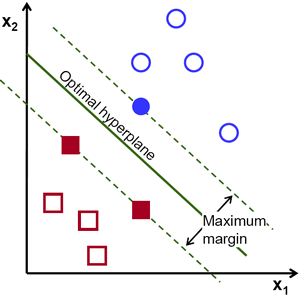
\includegraphics[scale=3.0]{margin-svm.png}
\caption{Siêu phẳng phân tách}
\label{fig:margin-svm}
\end{figure}
Khoảng cách từ một điểm đến siêu phẳng 
$$\frac{|<w.x_i>+b|}{||w||} $$
$$margin=d_+ +d_-=\frac{2}{||w||}$$ 
Tương đương bài toán cực tiểu hóa $\frac{<w.w>}{2}$ với điều kiện 
$$ \lbrace\begin{array}{l}
 <w.x_i>+b \geq 1 if y_i=1\\ <w.x_i>+b
    \leq -1  if y_i=-1 \end{array} $$
Áp dụng phương pháp Lagrange  
$$ L= 1/2 ||\overline{w}||^2 -\sum\alpha_i[y_i(\overline{w}.\overline{x_i} +b)-1] $$
Điều kiện 
$$ \frac{ \partial}{\partial\overline{w}}
=\overline{w}- \sum \alpha_i y_i x_i=0 \Longrightarrow \overline{w}=\sum \alpha_i y_i \overline{x_i} $$
$$\frac{ \partial}{\partial b}=-\sum \alpha_i y_i \Longrightarrow \sum x_i y_i=0$$ 
Thế vào ta được biểu thức :
$$L_D(\alpha)=\sum_{i=1}^r \alpha_i-1/2 \sum_{i,j=1}^{r}\alpha_i \alpha_j y_i y_j<x_i.x_j> $$
Điều kiện:
$$\{ \begin{array}{l}
\sum_{i=1 } ^{r} \alpha_i y_i =0 \\
\alpha_i \geq 0 \forall i=1..r
\end{array}
$$
Dung phương pháp lặp giải cuối cùng thu được
$$w^* =\sum_{x_i \in SV} \alpha_i y_i x_i  $$
$$b^*=y_k-<w*,x_k>$$
Để phân lớp cho giá trị mới ta tìm dấu của siêu phẳng $$ f(x)=\sum_{x_i \in SV} \alpha_i y_i <x_i .x>+b^*$$
Nới lỏng điểu kiện :
$$L_D(\alpha)=\sum_{i=1}^r \alpha_i-1/2 \sum_{i,j=1}^{r}\alpha_i \alpha_j y_i y_j<x_i.x_j> $$
$$
\{ \begin{array}{l}
\sum_{i=1 } ^{r} \alpha_i y_i =0 \\
0 \leq \alpha_i \leq C \forall i=1..r
\end{array}
$$
Phân lớp không tuyến tính một vài hàm nhân:\\
Đa thức $K(x,z)=(<x.z>+\Theta)^d $\\
Gaussian RBF $K(x,z)=e^{\frac{||x-z||^2}{2*\sigma}}$ trong đó $\sigma >0$\\
Phân lớp nhiều nhãn 2 chiến lược :
\begin{itemize}
\item one-versus-all
\item one-versus-one 
\end{itemize}
\section{Recurrent Neural Network (RNN)}
\subsection{RNN}
Recurrent Neural Network (RNN) là một mô hình phổ biến trong nhiều bài toán liên quan đến xử lý ngôn ngữ tự nhiên. Ý tưởng của RNN là sử dụng các thông tin liên tục (ghi nhớ các thông tin đã xử lý ở quá khứ). Sở dĩ RNN thích hợp cho bài toán xử lý ngông ngữ tự nhiên do ở mạng neuron truyền thống chúng ta giả sử tất cả các input sẽ được xử lý độc lập và đưa ra các output cũng độc lập với nhau. Mà các bài toán xử lý ngôn ngữ tự nhiên thì làm việc với đầu vào là các câu, các văn bản và mỗi câu trong văn bản hay mỗi từ trong một câu thì thường là không độc lập với nhau, chúng có mỗi liên hệ với nhau. Ví dụ với bài toán đoán từ tiếp theo trong câu thì để đoán được từ tiếp theo thì ta cần dựa vào các từ trước đó. Để giải quyết vấn đề đó, RNN sẽ xử lý các input theo thứ tự và đưa ra các output phụ thuộc vào các tính toán trước đó, hay nói cách khác RNN sẽ nhớ các thông tin trong quá khứ đã xử lý.
\par Mạng RNN có thể mô tả như hình vẽ dưới đây: 
\begin{figure}[H]
\centering
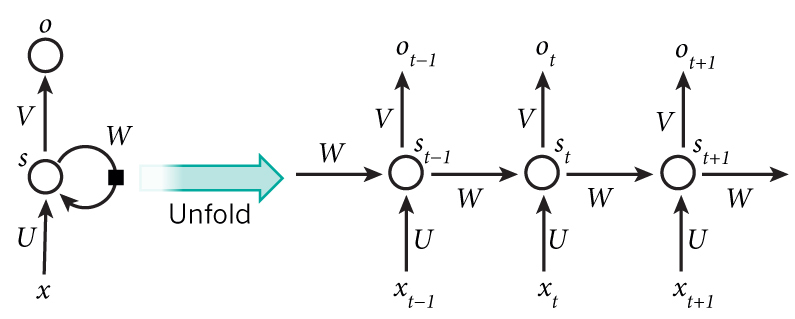
\includegraphics[scale=0.5]{rnn.jpg}
\caption{Mạng RNN}
\label{img_rnn}
\end{figure}
Trong hình \ref{img_rnn}:
\begin{itemize}
\item $x_t$ là input tại thời điểm t. Ví dụ: $x_0, x_1, x_2$ là one-hot vector của các từ 1, 2, 3 đầu vào.
\item $s_t$ là một trạng thái ẩn (trạng thái tạm thời, thông tin ghi nhớ). $s_t$ được tính phụ thuộc vào trạng thái ẩn phía trước và input của thời điểm hiện tại. $s_t = f(Ux_t + Ws_{t-1})$. Hàm f thường là hàm phi tuyến như \textbf{tanh} hoặc \textbf{ReLU}. $s_{-1}$ là đầu vào khi tính $s_0$ (trạng thái tạm thời đầu tiên), $s_{-1}$ thường bằng 0.
\item $o_t$ là output tại thời điểm t. Ví dụ: Nếu ta muốn đoán từ tiếp theo trong câu, $o_t$ là vector xác suất của các từ trong từ điển (nếu đầu vào là one-hot vector). $o_t = softmax(Vs_t)$
\end{itemize}
Các điều cần chú ý:
\begin{itemize}
\item Các bước tính toán sẽ được tính lần lượt. Ví dụ input đầu vào là một câu có 5 từ ($x_0, x_1, x_2, x_3, x_4$). Thì sau khi tính ra trạng thái ẩn ($s_0$) của từ thứ nhất ($x_0$) thì mới sử dụng thông tin $s_0, x_1$ để tính $s_1$. Các output $o_t$ có thể đưa ra hoặc không đưa ra ở mỗi bước tuỳ vào bài toán cụ thể: ví dụ ở bài toán phân tích quan điểm của một câu, ta chỉ cần đưa ra output cuối cùng (quan điểm của cả câu) mà không cần đưa ra các output ở mỗi bước (quan điểm của mỗi từ trong câu). Đặc trưng của RNN là các trạng thái ẩn, nơi mà giữ thông tin của các bước trước đó.  
\item Các trạng thái ẩn $s_t$ như là bộ nhớ (memory) của mạng RNN. $s_t$ sẽ giữ lại thông tin của các thời điểm phía trước. Output $o_t$ được tính toán dựa vào các thông tin đã ghi nhớ được tại thời điểm t.
\item Nếu như ở mạng neural truyền thống, mỗi tầng sẽ sử dụng các tham số khác nhau, thì ở RNN sẽ chia sẻ các tham số (U,W,V) ở tất cả các bước.
\end{itemize}

\subsubsection{Vấn đề Long-Term Dependencies}
Vấn đề  Long-Term Dependencies là vấn đề: trong xử lý tại bước hiện tại ta cần quá nhiều thông tin phụ thuộc không cần thiết của các bước trước.Một trong những đặc điểm nổi bật của RNN là mô hình này sẽ kết nối những thông tin phía trước để hỗ trợ cho bước xử lý hiện tại. Nhưng đôi khi ta chỉ cần dựa vào một số thông tin gần nhất để thực hiện bước xử lý hiện tại. Ví dụ trong bài toán đoán từ tiếp theo (\emph{sky}) trong đoạn văn có câu \emph{the clouds are in the sky} ta không cần những thông tin của quá nhiều từ trước đó ta vẫn có thể đoán được. Trong trường hợp này, khoảng cách tới cách thông tin liên quan được rút ngắn lại. Theo như mô hình chuẩn của RNN thì tất cả các thông tin của các bước phía trước đều được ghi nhớ lại và cung cấp cho bước xử lý hiện tại, dẫn đến việc dư thừa, không cần thiết. Vì vậy, mạng LSTM (Long Short Term Memory) đã xuất hiện để giải quyết vấn đề này.

\subsection{LSTM}
\subsubsection{Giới thiệu LSTM}
Mạng LSTM là một dạng đặc biệt của mạng RNN. LSTM được thiết kế để khắc phục vấn đề Long-Term Dependencies của RNN. 
\par Mô hình RNN chuẩn là việc lặp lại các module, các module này có cấu trúc đơn giản chỉ gồm một \textbf{tanh layer}.
\begin{figure}[H]
\centering
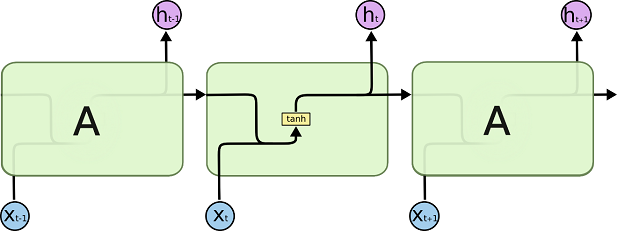
\includegraphics[scale=0.7]{rnn_tanh.jpg}
\caption{Mô hình RNN chuẩn với hàm tanh}
\end{figure}
\par LSTM cũng có cấu trúc lặp tương tự nhưng các module lặp có cấu trúc khác. Thay vì chỉ có một \textbf{tanh layer}, ta có bốn layer tương tác với nhau. 
\begin{figure}[H]
\centering
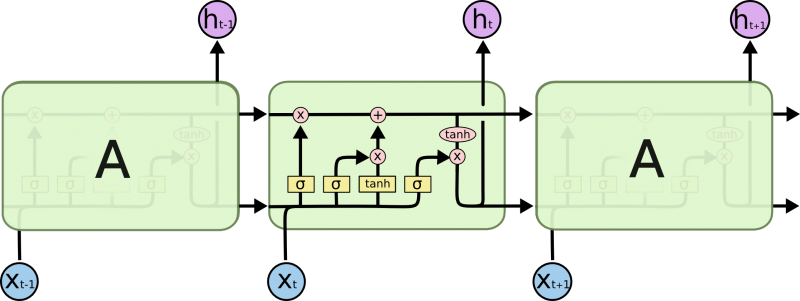
\includegraphics[scale=0.4]{lstm.png}
\caption{Mô hình LSTM}
\end{figure} 

\subsubsection{Ý tưởng chính của LSTM}
\par Điểm khác biệt lớn nhất của LSTM với RNN, đặc điểm nổi bật của LSTM chính là \textbf{cell state}. Cell state giống như một băng chuyền, nó chạy xuyên thẳng qua các module, ở mỗi module chỉ áp dụng một vài tương tác nhỏ tuyến tính (minor linear interaction). Điều này giúp cho thông tin ít bị thay đổi xuyên suốt quá trình lan truyền thông tin qua các bước.
\begin{figure}[H]
\centering
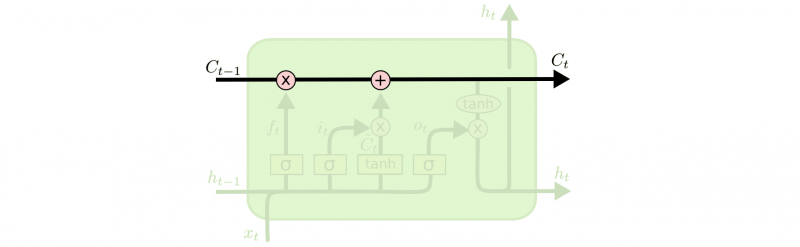
\includegraphics[scale=0.5]{lstm_cellstate.png}
\caption{LSTM với cell state}
\end{figure}
\par LSTM có khả năng thêm hoặc bớt các thông tin vào cell state, được quy định một cách cẩn thận bởi cấu trúc được gọi là cổng. Nhờ các cổng này ta có thể tùy chọn các thông tin sẽ được truyền đi cho bước kế tiếp. Chúng được tạo bởi sigmoid neural net layer và pointwise multiplication operation.
\begin{figure}[H]
\centering
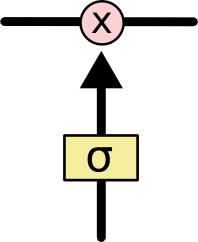
\includegraphics[scale=0.5]{lstm_gate.png}
\caption{LSTM gate}
\end{figure}
\par Hàm sigmoid có giá trị từ 0-1, mô tả độ lớn thông tin được phép truyền qua tại mỗi component.Nếu ta thu được 0 điều này có nghĩa là không cho bất kỳ thông tin nào đi qua, ngược lại nếu ta thu được 1 thì có nghĩa là cho phép mọi thứ đi qua. Một LSTM có ba cổng như vậy để bảo vệ và điều khiển cell state.

\subsubsection{Phân tích một module của LSTM}
\begin{figure}[H]
\centering
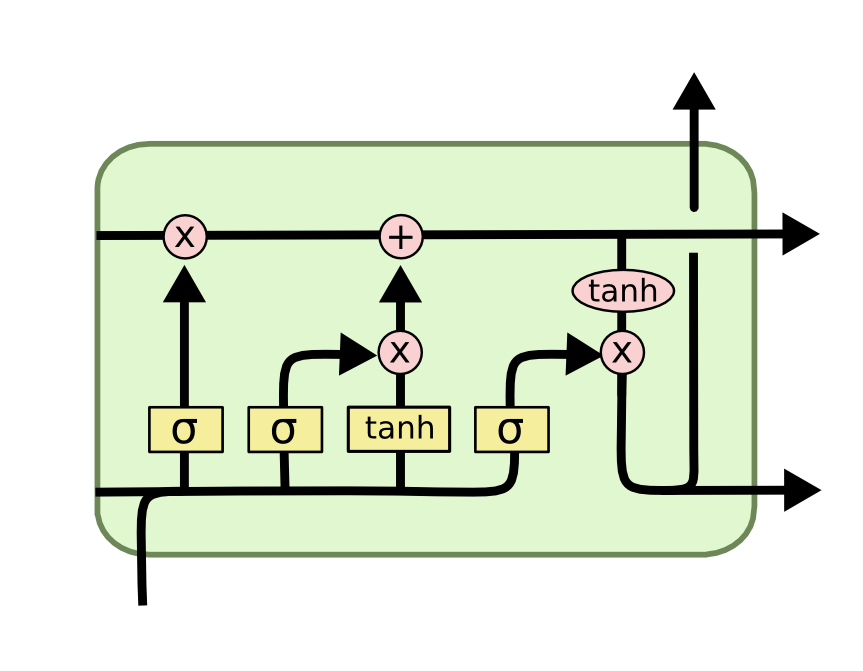
\includegraphics[scale=0.5]{lstm_module.png}
\caption{Một module của LSTM}
\end{figure}
\par Bước đầu tiên trong một module của LSTM là quyết định xem thông tin nào cần loại bỏ khỏi cell state. Quá trình này được thực hiện bởi một \emph{sigmoid layer} được gọi là \emph{forget gate layer}. Đầu vào là $h_{t-1}$ (thông tin đến từ bước trước đó) và $x_t$ (đầu vào tại bước hiện tại) và đầu ra là một số trong khoảng $[0,1]$. 1 là giữ lại toàn bộ thông tin, 0 là loại bỏ toàn bộ thông tin.
\begin{figure}[H]
\centering
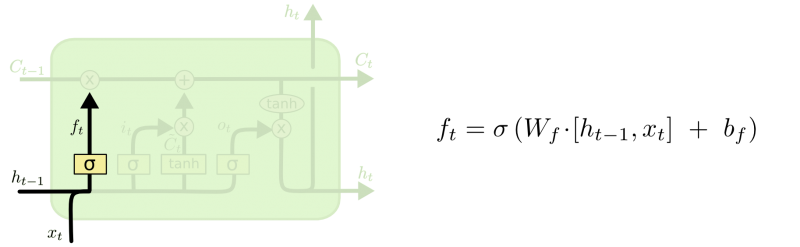
\includegraphics[scale=0.5]{lstm_module_firststep.png}
\caption{Forget gate layer}
\end{figure}
\par Bước tiếp theo là quyết định xem thông tin mới nào sẽ được lưu trữ trong cell state. Bước này gồm 2 phần. Đầu tiên, một \emph{sigmoid layer} cái được gọi là \emph{input gate layer} sẽ quyết định giá trị nào sẽ được cập nhật. Tiếp theo, một \emph{tanh layer} tạo ra vector các giá trị của các ứng cử viên mới $\tilde{C_t}$, cái sẽ được thêm vào cell state. 
\begin{figure}[H]
\centering
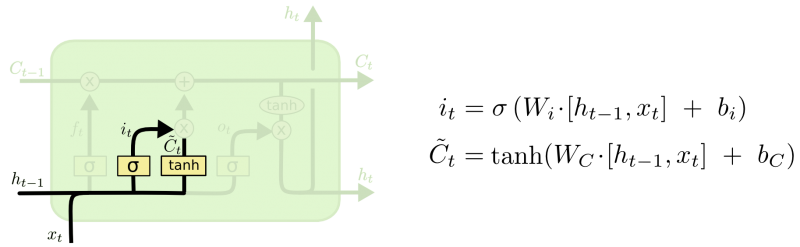
\includegraphics[scale=0.5]{lstm_module_secondstep.png}
\caption{Input gate layer}
\end{figure} 
\par Tiếp theo ta sẽ kết hợp 2 giá trị vừa được tạo để cập nhật vào cell state. Lúc cập nhật vào cell state cũ $C_{t-1}$ vào cell state mới $C_t$. Ta sẽ đưa hàm $f_t$ vào để quên đi những gì trước đó. Sau đó, thêm giá trị ứng viên mới $i_t*\tilde{C_t}$ để cập nhật cell state.
\begin{figure}[H]
\centering
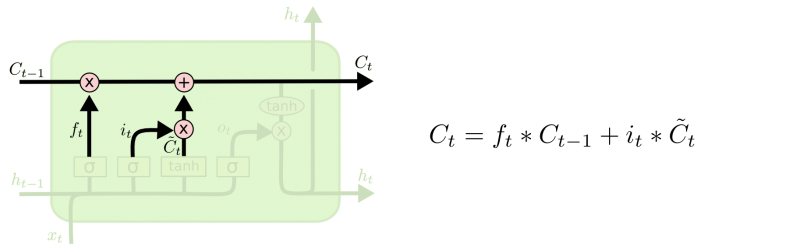
\includegraphics[scale=0.5]{lstm_module_update_cellstate.png}
\caption{Cập nhật cell state}
\end{figure}
\par Cuối cùng, ta cần quyết định xem thông tin output ra là gì. Output cần dựa trên cell state nhưng sẽ được lọc bớt. Đầu tiên, áp ụng \emph{sigmoid layer} để quyết định phần nào của cell state sẽ được output. Sau đó, đẩy cell state qua hàm \emph{tanh} và nhân với giá trị của các phần của cell state sẽ được giữ lại để output \emph{sigmoid layer} vừa tính trước đó.
\begin{figure}[H]
\centering
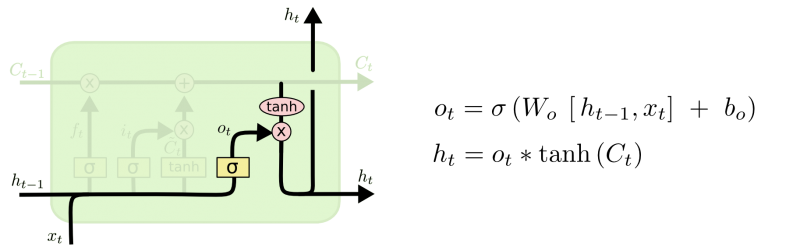
\includegraphics[scale=0.5]{lstm_module_output.png}
\caption{Output của một module}
\end{figure}



\chapter{Bài toán áp dụng}
\section{Giới thiệu bài toán}
Bài toán phân tích quan điểm là một trong những bài toán xử lý ngôn ngữ tự nhiên đang được áp dụng rộng rãi trong các ứng dụng lấy ý kiến phản hồi của khách hàng về các sản phẩm. Tương tự như bài toán phân loại văn bản, bài toán phân tích quan điểm cũng phân loại và gán nhán cho các đoạn văn, các câu văn. Bài toán có thể đơn giản chỉ có 2 nhãn như: tiêu cực, tích cực hoặc cũng có thể có nhiều nhãn: rất tích cực, tích cực, trung bình, tiêu cực, rất tiêu cực. 


\section{Kết quả thực nghiệm}


\subsection{SVM}
Bộ dữ liệu sử dụng là bộ tiwer với 10294 câu 3 nhãn.
Stopword có  424 từ
\begin{enumerate}
\item Xử lý dữ liệu loại bỏ url, tên riêng, các từ chưa đúng bằng biểu thức chính quy
\item Sử dụng biểu diễn từ one-hot vector
\item Sử dụng thư viện hỗ trợ trên ngôn ngữ python regex,sklearn, csv
\item Tham số mô hình C=1.0 hàm nhân: linear chế độ one vs one 
\item Tập train 8000 tập test 1924
\item Kết quả đạt được khoảng 66$\%$
\end{enumerate}


\subsection{LSTM}
Bộ dữ liệu sử dụng là bộ dữ liệu IMDB. Bộ dữ liệu bao gồm các câu đánh giá phim và bao gồm 2 nhãn. Bộ dữ liệu bao gồm 25000 review cho training và 25000 reviews cho bộ test. Bài toán yêu cầu xác định một câu đánh giá phim là tích cực hay tiêu cực.

Sử dụng thư viện keras:
\begin{enumerate}
\item Mô hình hóa dữ liệu
\begin{itemize}
\item Mỗi đánh giá phim chỉ lấy 500 từ. Nếu đánh giá nào có số từ dài hơn sẽ bị chặt bớt còn nếu đánh giá nào có ít từ hơn sẽ chèn thêm các số 0.
\item Chiều của word embedded vector là 32.
\end{itemize}
\item Training: Mô hình áp dụng:
$$ INPUT \rightarrow WordEmbedding \rightarrow LSTM \rightarrow sigmoid \rightarrow output$$
\begin{itemize}
\item Đầu vào là câu gồm 500 từ
\item Chuyển thành 500 vector số thực 32 chiều.
\item Mỗi vector là đầu vào của một module trong LSTM, và 100 module cuối cùng đưa ra output 
\item Output của 100 module đưa vào neuron với hàm tác động là sigmoid để đưa ra output là 0 hoặc 1 (tiêu cực hay tích cực)
\end{itemize}
\item Môi trường thực nghiệm:
\begin{itemize}
\item Hệ điều hành Unbutun 16.04 64 bit
\item Intel Core i5-4210U CPU 1.70GHz $\times$ 4
\item Ngôn ngữ lập trình Python
\item Thư viện hỗ trợ Keras
\end{itemize}
\item Kết quả: Độ chính xác 84.97\%
\\[0.5cm]{\small
Epoch 1/3\\
25000/25000 [======================] - 498s - loss: 0.5891 - acc: 0.6910\\
Epoch 2/3\\
25000/25000 [======================] - 472s - loss: 0.3168 - acc: 0.8696\\   
Epoch 3/3\\
25000/25000 [======================] - 466s - loss: 0.2502 - acc: 0.9026\\
Accuracy: 84.97\% \\
}
\end{enumerate}

\chapter{Kết luận}
Dựa vào kết quả thư được sau quá trình thử nghiệm chúng em nhận thấy rằng SVM và mạng LSTM là hai phương pháp hiệu quả cho bài toán phân tích quan điểm. Mạng LTSM là phương pháp ra đời sau nhưng thể hiện được hiệu quả vượt trội cũng như là một ngôi sao sáng trong DeepLearning. SVM là một phương pháp học máy truyền thống cũng hiệu quả cho các bài toán liên quan đến ngôn ngũ tự nhiên. 
\section{Khó khăn gặp phải}
\begin{itemize}
\item Cài đặt trên ngôn ngữ python
\item Tài nguyên máy không cho phép xử lý với các bộ dữ liệu lớn

\end{itemize}
\section{Những điều chưa đạt được}
\begin{itemize}
\item Thư nghiệm nhiều hơn các phương pháp chọn đặc trưng cho SVM
\item Cho các phương pháp chạy trên cùng một tập dữ liệu để so sánh 
\end{itemize}

\begin{thebibliography}{9}
\bibitem{1} \url{http://www.wildml.com/2015/09/recurrent-neural-networks-tutorial-part-1-introduction-to-rnns/}
\bibitem{2} \url{http://colah.github.io/posts/2015-08-Understanding-LSTMs/}
\bibitem{3} \url{http://cs224d.stanford.edu/syllabus.html}
\bibitem{4} \url{https://ongxuanhong.wordpress.com/2016/09/16/long-short-term-memory-lstm/}
\bibitem{5} \url{https://www.ravikiranj.net/posts/2012/code/how-build-twitter-sentiment-analyzer/}
\bibitem{5} \url{http://scikit-learn.org/stable/modules/svm.html}
\end{thebibliography}


\end{document}
